\subsection{Overview}
This section explains how the BBP system components are implemented and integrated, and in what order the different parts are developed and brought together. The goal is to reduce technical risk by following an incremental approach that enables continuous testing throughout development. The proposed strategy also considers dependencies between components and the priorities set by the functional requirements, making it easier for the development team to work in parallel. The different testing levels are also described. They are used to verify that the implementation aligns with the architectural design and meets all requirements specified in the RASD.

\subsection{Implementation Strategy}
The implementation of the BBP system follows an incremental approach based on the dependencies between the components and on the priority of the functional requirements. The adopted strategy employs bottom-up development, starting from the more internal layers toward the external ones, with continuous integration of the completed components.
The proposed implementation order is:
\begin{enumerate}
    \item \textbf{Data Layer}: PostgreSQL database configuration with PostGIS extension, schema definition and implementation of the Repositories
    \item \textbf{Core Services}: Development of the business logic services that do not depend on external services (Authentication Service, User Management Service)
    \item \textbf{External Integration Services}: Implementation of the adapters for Mapbox and Open-Meteo
    \item \textbf{Domain Services}: Development of the services that orchestrate the domain logic (Trip Service, Bike Path Service, Obstacle Management Service)
    \item \textbf{Specialized Services}: Implementation of Bike Path Finder Service and Sensor Analysis Service
    \item \textbf{Controller Layer}: Exposure of the REST APIs
    \item \textbf{Frontend}: Development of the web application (Vue.js) and mobile application (Flutter)
\end{enumerate}
This strategy allows testing each component in isolation before the integration and facilitates parallel work on independent components.

\subsubsection{Features Identification}
The functionalities of the system have been grouped into incremental features, each of which implements a coherent subset of requirements:
\begin{itemize}
    \item \textbf{F1 - User Management}: Registration, login, logout, profile management (R1–R4)
    \item \textbf{F2 - Manual Trip Recording}: Manual insertion of trips with automatic calculation of statistics and weather enrichment (R5–R7, R9–R10)
    \item \textbf{F3 - Manual Bike Path Creation}: Manual creation of routes with obstacle management and quality score calculation (R11, R13–R18)
    \item \textbf{F4 - Bike Path Search}: Search for public routes with ordering by quality (R19–R20)
    \item \textbf{F5 - Collaborative Maintenance}: Reporting and modification of obstacles with automatic recalculation of quality score (R21–R23)
    \item \textbf{F6 - Automatic Trip Recording}: Automatic tracking of trips via GPS (R8)
    \item \textbf{F7 - Automatic Bike Path Creation}: Automatic creation of routes with obstacle detection through sensors and user validation (R12)
\end{itemize}
The implementation order of the features follows the dependencies among the various parts of the system: F1 is developed first because it is a prerequisite for all the other features that require authentication. F2 and F3 are implemented before F6 and F7, so as to first validate the basic functionalities and introduce only in a second moment the more complex automatic capabilities.

\subsection{Component Integration}
The integration of the components follows the implementation order defined by the bottom-up strategy. Each component, once completed and unit tested, is integrated with those already present in the system, in order to immediately verify the interactions between the different layers. \\
For each feature indicated in section 5.1.1, an integration diagram is provided that shows the order in which the components are implemented, integrated, and tested. Even though the bottom-up approach could lead to developing related modules in parallel, the diagrams are organized by feature to make them clearer to read. \\
The PostgreSQL database with PostGIS is configured from the beginning and it is assumed to remain available during the integration of the subsequent features. The external services (Mapbox, Open-Meteo) do not appear in the diagrams because they operate independently of the BBP system; during development, however, mocks are used to test the integration before connecting to the real APIs. \\
The diagrams highlight the gradual addition of components: Repositories, Services, and Controllers are integrated step by step until the completion of each feature. \\

\textbf{[F1] User Management} \\
\begin{figure}[h!]
    \centering
        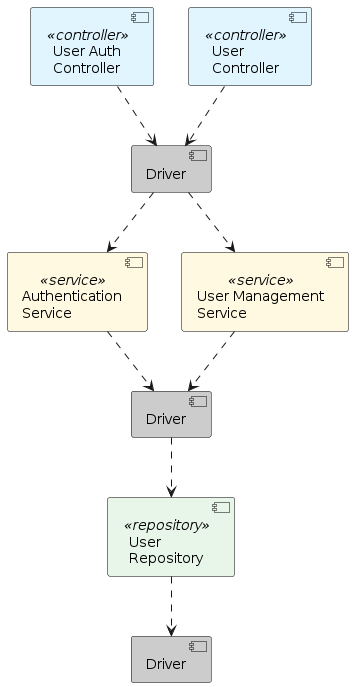
\includegraphics[width=\linewidth]{DD/images/f1-test.png}
    \caption{Integration Diagram: User Management}
    \label{fig:f1-test}
\end{figure}
The diagram shows the integration strategy for the User Management feature. The User Repository is implemented first, together with the drivers needed to test it in isolation. Subsequently, the Authentication Service and the User Management Service, which depend on the Repository, are integrated. Finally, the User Auth Controller and the User Controller are added, which expose the functionalities via REST APIs.

\textbf{[F2] Manual Trip Recording} \\
\begin{figure}[h!]
    \centering
        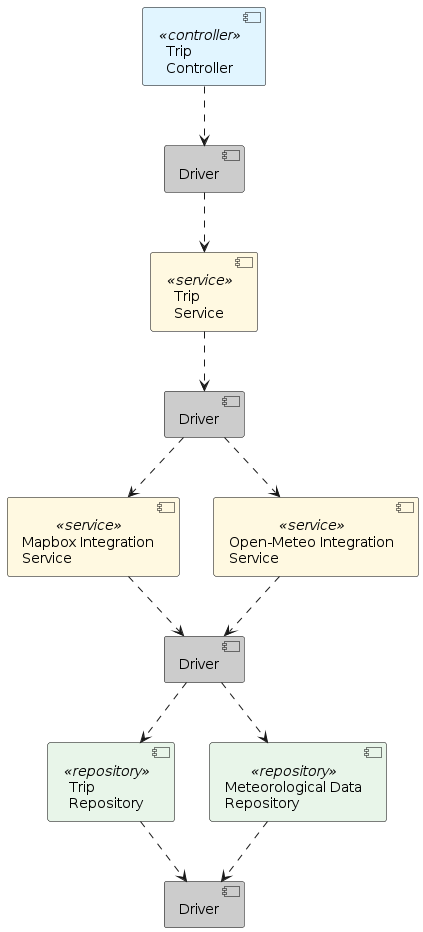
\includegraphics[width=\linewidth]{DD/images/f2-test.png}
    \caption{Integration Diagram: Manual Trip Recording}
    \label{fig:f2-test}
\end{figure}
The diagram describes how the Manual Trip Recording feature is integrated. It starts from the “lower” layers, first implementing the Trip Repository and the Meteorological Data Repository. Then the external services Mapbox Integration Service and Open-Meteo Integration Service are integrated, used respectively for route calculation and for weather data. At this point the Trip Service comes into play, which manages the domain logic by coordinating repositories and external services. Finally, the Trip Controller exposes the functionalities through REST APIs.

\textbf{[F3] Manual Bike Path Creation} \\
\begin{figure}[h!]
    \centering
        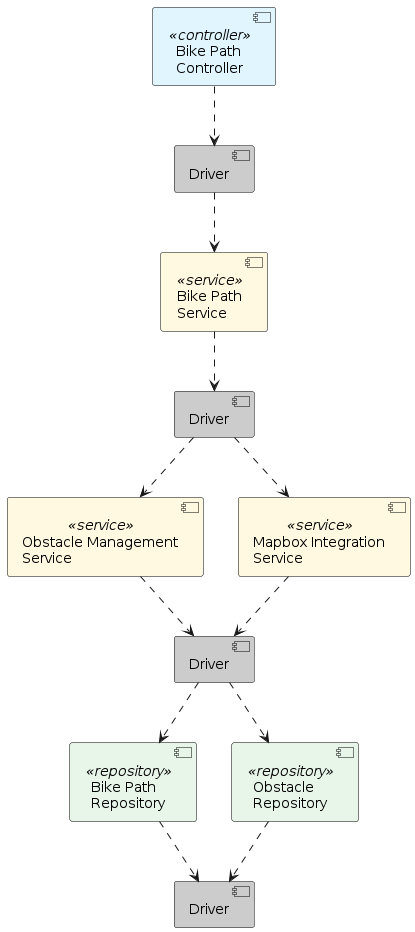
\includegraphics[width=\linewidth]{DD/images/f3-test.png}
    \caption{Integration Diagram: Manual Bike Path Creation}
    \label{fig:f3-test}
\end{figure}
The diagram shows the integration for Manual Bike Path Creation. It starts from the Bike Path Repository and the Obstacle Repository. Then the Mapbox Integration Service is integrated for geometry calculation and the Obstacle Management Service for obstacle validation. The Bike Path Service coordinates path creation, obstacle management, and quality score calculation. Finally, the Bike Path Controller exposes the APIs.

\textbf{[F4] Bike Path Search} \\
\begin{figure}[h!]
    \centering
        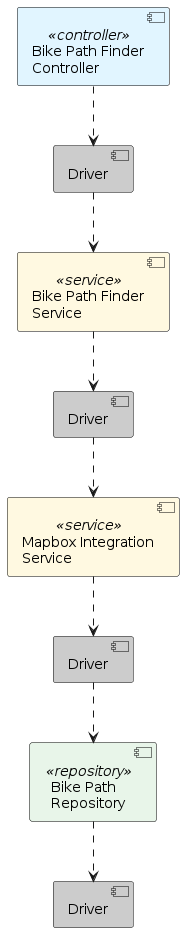
\includegraphics[width=\linewidth]{DD/images/f4-test.png}
    \caption{Integration Diagram: Bike Path Search}
    \label{fig:f4-test}
\end{figure}
The diagram shows the integration for Bike Path Search. The Bike Path Repository is implemented first to access public paths. Then the Mapbox Integration Service is integrated for address geocoding. The Bike Path Finder Service performs spatial queries and sorts results by quality score. Finally, the Bike Path Finder Controller exposes the search API.

\textbf{[F5] Collaborative Maintenance} \\
\begin{figure}[h!]
    \centering
        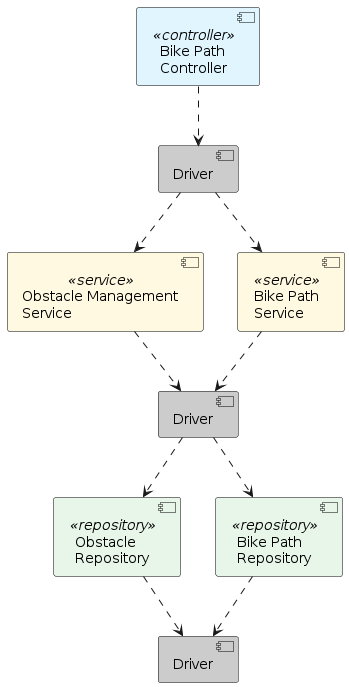
\includegraphics[width=\linewidth]{DD/images/f5-test.png}
    \caption{Integration Diagram: Collaborative Maintenance}
    \label{fig:f5-test}
\end{figure}
The diagram shows the integration for Collaborative Maintenance. It starts from the Obstacle Repository and the Bike Path Repository. The Obstacle Management Service handles obstacle creation and modification, while the Bike Path Service recalculates the quality score. The Bike Path Controller exposes the APIs for reporting and updating obstacles.

\textbf{[F6] Automatic Trip Recording} \\
\begin{figure}[h!]
    \centering
        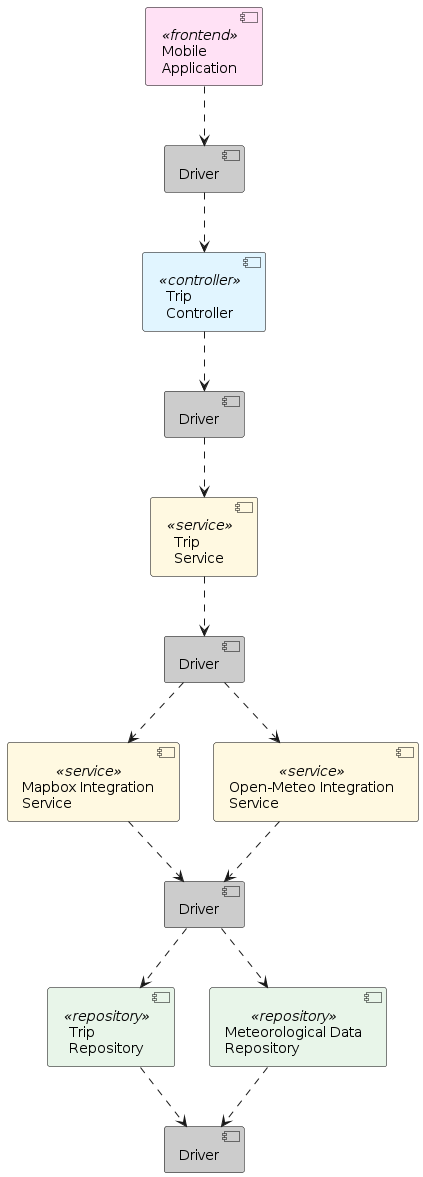
\includegraphics[width=\linewidth]{DD/images/f6-test.png}
    \caption{Integration Diagram: Automatic Trip Recording}
    \label{fig:f6-test}
\end{figure}
The diagram shows the integration for Automatic Trip Recording. The components of F2 are reused, adding the Mobile Application that tracks the route via GPS in real time and sends the data to the backend through the Trip Controller.

\textbf{[F7] Automatic Bike Path Creation} \\
\begin{figure}[h!]
    \centering
        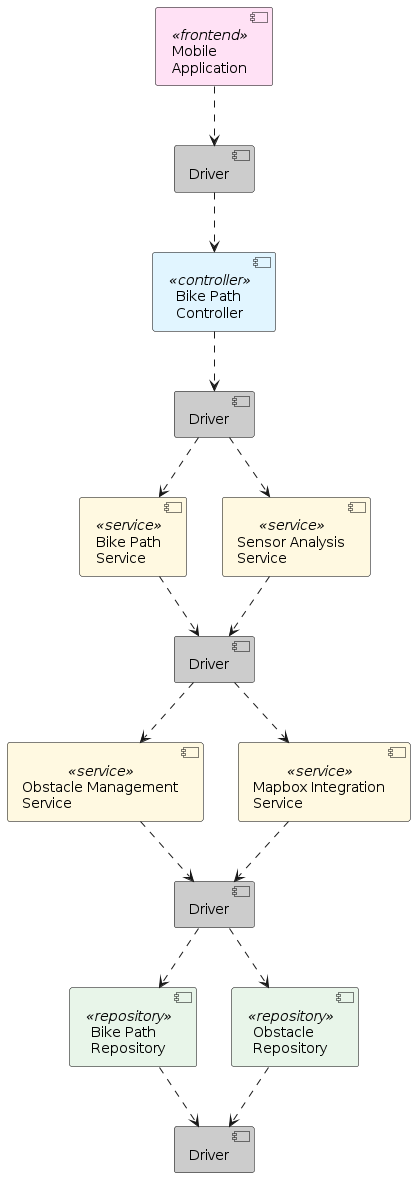
\includegraphics[width=\linewidth]{DD/images/f7-test.png}
    \caption{Integration Diagram: Automatic Bike Path Creation}
    \label{fig:f7-test}
\end{figure}
The diagram shows the integration for Automatic Bike Path Creation. The components of F3 are reused, adding the Mobile Application that tracks GPS and detects obstacles through sensors. The Sensor Analysis Service validates and enriches the detected anomalies with a confidence score and cross-validation before the user confirms the creation of the path.


\subsection{Test Plan}
The test plan describes the different types of tests needed to verify that the implementation is correct and that it complies with the requirements. \\
\textbf{Unit Testing}: each component is tested individually to check its behavior. The Services are verified using mocks of the Repositories and of the external services, the Repositories with an in-memory database, and the Controllers by simulating the underlying Services. \\
\textbf{Integration Testing}: after the unit tests, the components are connected to each other and tested together. The interactions between Controllers and Services, between Services and Repositories, and between Services and external services are checked; for Mapbox and Open-Meteo, mocks are used that reproduce the API responses. In addition, the complete REST API flows are tested, verifying that the data passes correctly through all layers. \\
\textbf{System Testing}: once the integration is completed, the entire system is tested to verify that all functionalities are implemented correctly and that the functional and non-functional requirements defined in the RASD are respected. \\
This includes the following test types:
\begin{itemize}
    \item \textbf{Functional Testing}: helps make sure the system meets all functional requirements. The end-to-end use cases, as defined in the RASD, are tested to confirm that each feature (F1–F7) works as expected
    \item \textbf{Performance Testing}: focuses on assessing system performance and spotting any bottlenecks. The efficiency of PostGIS spatial queries, API response times, and the mobile app’s performance during GPS tracking are checked
    \item \textbf{Load Testing}: helps understand how the system behaves under load. It tests the ability to handle simultaneous requests and steadily increasing data volumes, while also evaluating the scalability of the stateless architecture
    \item \textbf{Stress Testing}: pushes the system under extreme conditions to find its limits and verify graceful degradation. It also simulates external service outages to ensure error handling works properly
\end{itemize}

\subsection{Additional Specifications on Testing}
The testing process also includes validation activities with real users, in order to verify that the system truly meets stakeholders’ expectations. User acceptance testing is therefore carried out through iterative cycles of feedback and subsequent corrections. \\
The implementation includes two phases of user testing: an alpha phase, with a small group made up of the development team and some selected stakeholders, followed by a beta phase with a larger sample of end users under real usage conditions. In this way, it is possible to identify any critical issues in a controlled environment, before making the system available to a wider audience. \\
The introduction of new functionalities after the initial release follows an incremental deployment strategy. The features are released progressively, starting from a limited number of users and gradually expanding availability until it covers the entire base. This approach makes it possible to measure the real impact of the changes and to intervene quickly in case of anomalies, reducing the risk for the overall user base. \\
Stakeholder feedback is collected systematically throughout the entire system life cycle and helps bring out usability issues or bugs that may not have been caught by automated tests. Every new addition or modification requires the full execution of the test suite, in order to verify the absence of regressions. \\
All testing activities are documented according to industry standards, ensuring full traceability of issues found, solutions adopted, and decisions made throughout the entire process.